\documentclass{beamer}

\usepackage[utf8]{inputenc}
\input{../helper}

\title{Introdução à Computação \\ alocação dinâmica de memória}
\author{Alexandre Rademaker}
\date{}

\begin{document}

\begin{frame}
 \maketitle
\end{frame}

\begin{frame}[fragile,allowframebreaks]{alocação dinâmica de memória}

  Vimos como declarar ponteiros e \textbf{apontá-los} para variáveis
  já existentes. Isto é, preencher seu valor com endereços já
  alocados na memória.

  Em vários problemas que vimos até agora, alocamos trechos de memória
  além do necessário exatamente por não saber a quantidade
  de memória exatamente necessária durante a compilação.

  Em alguns casos a quantidade de memória necessária não é conhecida
  no momento da compilação mas apenas no tempo de execução. (ex: lendo
  um arquivo)

  \framebreak

  Podemos atribuir novos endereços de memória para ponteiros também,
  endereços alocados de forma dinâmica, durante a execução do programa.

  Memória alocada de forma dinâmica vem de um espaço conhecido como
  \textbf{heap}.

  Até agora, só usávamos memória da área conhecida como
  \textbf{stack}.

  \framebreak

  \begin{center}
    
\includegraphics[width=.7\textwidth]{stack-heap.png}
  \end{center}

  \framebreak

  Para alocar memória de maneira dinâmica, usamos a função
  \ilcode{malloc()} da biblioteca C standard library, passando para
  ela o número de \textbf{bytes} necessários.

  A função \ilcode{malloc()} retorna um ponteiro para a nova região
  alocada. Se \ilcode{malloc()} não conseguir alocar a memória
  solicitada, irá retornar \ilcode{NULL}.

  \framebreak

  \begin{lstlisting}[style=normalc]
    // alocacao estatica
    int x;
    
    // alocacao dinamica
    int *px = malloc(4);
  \end{lstlisting}

  \framebreak

  \begin{lstlisting}[style=normalc]
    // alocacao estatica
    int x;
    
    // alocacao dinamica
    int *px = malloc(sizeof(int));
  \end{lstlisting}

  O operador \ilcode{sizeof} retorna o tamanho que um tipo que recebe
  como argumento. Também podemos passar uma variável ou expressão para
  o \ilcode{sizeof} para obter o tamanho ocupado por ela.

  \framebreak

  \begin{lstlisting}[style=normalc]
    // lendo um valor do usuario
    int x = get_int_from_user();
    
    // array de x elementos float na stack
    float arr1[x];
    
    // array de x elementos float no heap
    float* arr2 = malloc(x * sizeof(float));
  \end{lstlisting}

  \framebreak

  Mas temos um problema!

  Memória alocada de forma dinâmica não é controlada pelo sistema e
  não é automaticamente liberada quando o escopo onde ela foi
  declarada termina.

  Se a memória não for liberada, temos o que chamamos de
  \textbf{memory leak}.  Memória perdida que o sistema não sabe que
  poderia usar, logo a performace do sistema pode degradar.

  O programador deve, quando terminar de usar a memória, liberá-la com
  a função \ilcode{free()}.

  \framebreak

  \begin{lstlisting}[style=normalc]
    // alocacao dinamica
    int *px = malloc(sizeof(int));

    // faz alguma coisa

    // liberando
    free(px);
  \end{lstlisting}

  \framebreak

  Regras importantes

  \begin{itemize}
  \item todo bloco de memória alocado com \ilcode{malloc()} deve ser liberado com \ilcode{free()}.
  \item apenas memória alocada com o \ilcode{malloc()} pode ser liberada com \ilcode{free()}.
  \item não tente liberar o mesmo bloco de memória duas vezes.
  \end{itemize}

\end{frame}


\begin{frame}[allowframebreaks,fragile]{alocação dinâmica}

  \begin{columns}
    \begin{column}{.5\textwidth}
      {\texttt
        int m;
      }
    \end{column}
    \begin{column}{.5\textwidth}
      \begin{tikzpicture}[scale=1]
        % \draw[help lines, gray!50, very thin] (0,0) grid (4,4);
        % \filldraw[black] (0,0) circle (2pt);
        
        % \draw[fill=green!40, rounded corners=5pt] (3,3) rectangle node {\textbf{ }} (4,4);

        % \draw[fill=green!40, rounded corners=5pt] (0,3) rectangle node {\textbf{ }} (1,4);
        % \node at (0.5,2.7) {m};

        % \draw[fill=green!20, rounded corners=5pt] (3,0) rectangle node {\textbf{ }} (4,1);
        % \node at (3.5,-0.3) {b};
        % \draw[->, very thick] (3.5,0.5) -- (3.5,3);

        % \draw[fill=green!20, rounded corners=5pt] (0,0) rectangle node {\textbf{ }} (1,1);
        % \node at (0.5,-0.3) {a};
        % \draw[->, very thick] (0.7,0.5) -- (0.7,3);
      \end{tikzpicture}      
    \end{column}
  \end{columns}

  \framebreak    

  \begin{columns}
    \begin{column}{.5\textwidth}
      {\texttt
        int m;
      }
    \end{column}
    \begin{column}{.5\textwidth}
      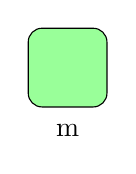
\begin{tikzpicture}[scale=1]
        % \draw[help lines, gray!50, very thin] (0,0) grid (4,4);
        % \filldraw[black] (0,0) circle (2pt);
        
        % \draw[fill=green!40, rounded corners=5pt] (3,3) rectangle node {\textbf{ }} (4,4);

        \draw[fill=green!40, rounded corners=5pt] (0,3) rectangle node {\textbf{ }} (1,4);
        \node at (0.5,2.7) {m};

        % \draw[fill=green!20, rounded corners=5pt] (3,0) rectangle node {\textbf{ }} (4,1);
        % \node at (3.5,-0.3) {b};
        % \draw[->, very thick] (3.5,0.5) -- (3.5,3);

        % \draw[fill=green!20, rounded corners=5pt] (0,0) rectangle node {\textbf{ }} (1,1);
        % \node at (0.5,-0.3) {a};
        % \draw[->, very thick] (0.7,0.5) -- (0.7,3);
      \end{tikzpicture}      
    \end{column}
  \end{columns}

  \framebreak    

  \begin{columns}
    \begin{column}{.5\textwidth}
      {\texttt
        int m;\\
        int* a;
      }
    \end{column}
    \begin{column}{.5\textwidth}
      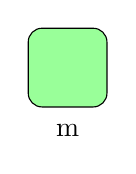
\begin{tikzpicture}[scale=1]
        % \draw[help lines, gray!50, very thin] (0,0) grid (4,4);
        % \filldraw[black] (0,0) circle (2pt);
        
        % \draw[fill=green!40, rounded corners=5pt] (3,3) rectangle node {\textbf{ }} (4,4);

        \draw[fill=green!40, rounded corners=5pt] (0,3) rectangle node {\textbf{ }} (1,4);
        \node at (0.5,2.7) {m};

        % \draw[fill=green!20, rounded corners=5pt] (3,0) rectangle node {\textbf{ }} (4,1);
        % \node at (3.5,-0.3) {b};
        % \draw[->, very thick] (3.5,0.5) -- (3.5,3);

        % \draw[fill=green!20, rounded corners=5pt] (0,0) rectangle node {\textbf{ }} (1,1);
        % \node at (0.5,-0.3) {a};
        % \draw[->, very thick] (0.7,0.5) -- (0.7,3);
      \end{tikzpicture}      
    \end{column}
  \end{columns}

  \framebreak    

  \begin{columns}
    \begin{column}{.5\textwidth}
      {\texttt
        int m;\\
        int* a;
      }
    \end{column}
    \begin{column}{.5\textwidth}
      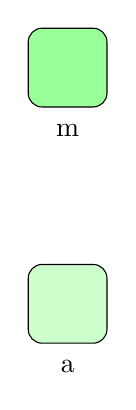
\begin{tikzpicture}[scale=1]
        % \draw[help lines, gray!50, very thin] (0,0) grid (4,4);
        % \filldraw[black] (0,0) circle (2pt);
        
        % \draw[fill=green!40, rounded corners=5pt] (3,3) rectangle node {\textbf{ }} (4,4);

        \draw[fill=green!40, rounded corners=5pt] (0,3) rectangle node {\textbf{ }} (1,4);
        \node at (0.5,2.7) {m};

        % \draw[fill=green!20, rounded corners=5pt] (3,0) rectangle node {\textbf{ }} (4,1);
        % \node at (3.5,-0.3) {b};
        % \draw[->, very thick] (3.5,0.5) -- (3.5,3);

        \draw[fill=green!20, rounded corners=5pt] (0,0) rectangle node {\textbf{ }} (1,1);
        \node at (0.5,-0.3) {a};
        % \draw[->, very thick] (0.7,0.5) -- (0.7,3);
      \end{tikzpicture}      
    \end{column}
  \end{columns}

  \framebreak    

  \begin{columns}
    \begin{column}{.5\textwidth}
      {\texttt
        int m;\\
        int* a;\\
        int* b = malloc(sizeof(int));
      }
    \end{column}
    \begin{column}{.5\textwidth}
      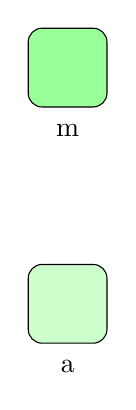
\begin{tikzpicture}[scale=1]
        % \draw[help lines, gray!50, very thin] (0,0) grid (4,4);
        % \filldraw[black] (0,0) circle (2pt);
        
        % \draw[fill=green!40, rounded corners=5pt] (3,3) rectangle node {\textbf{ }} (4,4);

        \draw[fill=green!40, rounded corners=5pt] (0,3) rectangle node {\textbf{ }} (1,4);
        \node at (0.5,2.7) {m};

        % \draw[fill=green!20, rounded corners=5pt] (3,0) rectangle node {\textbf{ }} (4,1);
        % \node at (3.5,-0.3) {b};
        % \draw[->, very thick] (3.5,0.5) -- (3.5,3);

        \draw[fill=green!20, rounded corners=5pt] (0,0) rectangle node {\textbf{ }} (1,1);
        \node at (0.5,-0.3) {a};
        % \draw[->, very thick] (0.7,0.5) -- (0.7,3);
      \end{tikzpicture}      
    \end{column}
  \end{columns}

  \framebreak    

  \begin{columns}
    \begin{column}{.5\textwidth}
      {\texttt
        int m;\\
        int* a;\\
        int* b = malloc(sizeof(int));
      }
    \end{column}
    \begin{column}{.5\textwidth}
      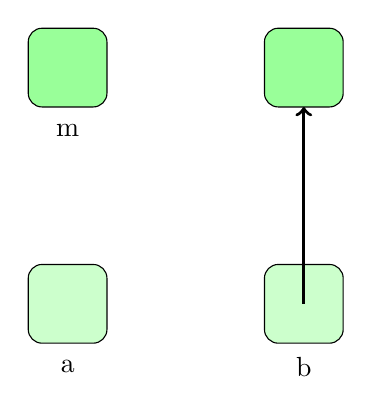
\begin{tikzpicture}[scale=1]
        % \draw[help lines, gray!50, very thin] (0,0) grid (4,4);
        % \filldraw[black] (0,0) circle (2pt);
        
        \draw[fill=green!40, rounded corners=5pt] (3,3) rectangle node {\textbf{ }} (4,4);

        \draw[fill=green!40, rounded corners=5pt] (0,3) rectangle node {\textbf{ }} (1,4);
        \node at (0.5,2.7) {m};

        \draw[fill=green!20, rounded corners=5pt] (3,0) rectangle node {\textbf{ }} (4,1);
        \node at (3.5,-0.3) {b};
        \draw[->, very thick] (3.5,0.5) -- (3.5,3);

        \draw[fill=green!20, rounded corners=5pt] (0,0) rectangle node {\textbf{ }} (1,1);
        \node at (0.5,-0.3) {a};
        % \draw[->, very thick] (0.7,0.5) -- (0.7,3);
      \end{tikzpicture}      
    \end{column}
  \end{columns}

  \framebreak    

  \begin{columns}
    \begin{column}{.5\textwidth}
      {\texttt
        int m;\\
        int* a;\\
        int* b = malloc(sizeof(int));\\
        a = \&m;\\
      }
    \end{column}
    \begin{column}{.5\textwidth}
      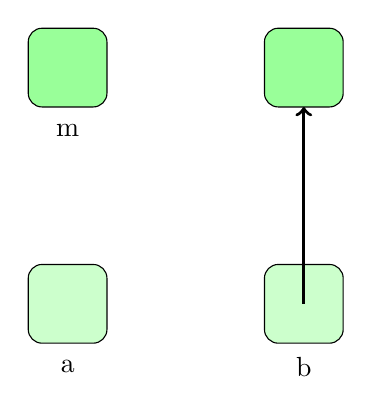
\begin{tikzpicture}[scale=1]
        % \draw[help lines, gray!50, very thin] (0,0) grid (4,4);
        % \filldraw[black] (0,0) circle (2pt);
        
        \draw[fill=green!40, rounded corners=5pt] (3,3) rectangle node {\textbf{ }} (4,4);

        \draw[fill=green!40, rounded corners=5pt] (0,3) rectangle node {\textbf{ }} (1,4);
        \node at (0.5,2.7) {m};

        \draw[fill=green!20, rounded corners=5pt] (3,0) rectangle node {\textbf{ }} (4,1);
        \node at (3.5,-0.3) {b};
        \draw[->, very thick] (3.5,0.5) -- (3.5,3);

        \draw[fill=green!20, rounded corners=5pt] (0,0) rectangle node {\textbf{ }} (1,1);
        \node at (0.5,-0.3) {a};
        % \draw[->, very thick] (0.7,0.5) -- (0.7,3);
      \end{tikzpicture}      
    \end{column}
  \end{columns}

  \framebreak    

  \begin{columns}
    \begin{column}{.5\textwidth}
      {\texttt
        int m;\\
        int* a;\\
        int* b = malloc(sizeof(int));\\
        a = \&m;\\
      }
    \end{column}
    \begin{column}{.5\textwidth}
      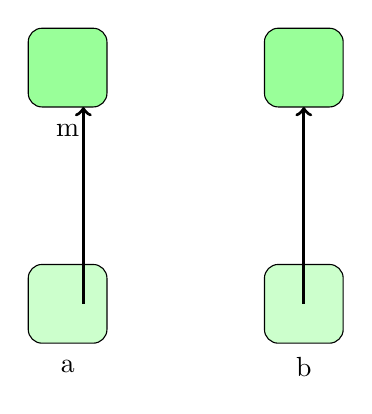
\begin{tikzpicture}[scale=1]
        % \draw[help lines, gray!50, very thin] (0,0) grid (4,4);
        % \filldraw[black] (0,0) circle (2pt);
        
        \draw[fill=green!40, rounded corners=5pt] (3,3) rectangle node {\textbf{ }} (4,4);

        \draw[fill=green!40, rounded corners=5pt] (0,3) rectangle node {\textbf{ }} (1,4);
        \node at (0.5,2.7) {m};

        \draw[fill=green!20, rounded corners=5pt] (3,0) rectangle node {\textbf{ }} (4,1);
        \node at (3.5,-0.3) {b};
        \draw[->, very thick] (3.5,0.5) -- (3.5,3);

        \draw[fill=green!20, rounded corners=5pt] (0,0) rectangle node {\textbf{ }} (1,1);
        \node at (0.5,-0.3) {a};
        \draw[->, very thick] (0.7,0.5) -- (0.7,3);
      \end{tikzpicture}      
    \end{column}
  \end{columns}

  \framebreak    

  \begin{columns}
    \begin{column}{.5\textwidth}
      {\texttt
        int m;\\
        int* a;\\
        int* b = malloc(sizeof(int));\\
        a = \&m;\\
        a = b;
      }
    \end{column}
    \begin{column}{.5\textwidth}
      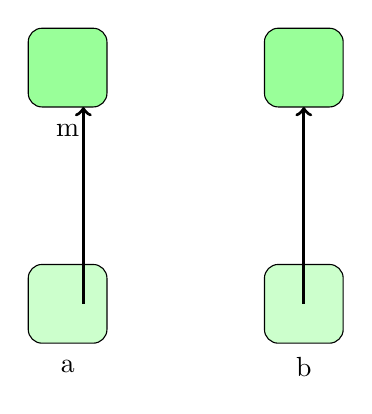
\begin{tikzpicture}[scale=1]
        % \draw[help lines, gray!50, very thin] (0,0) grid (4,4);
        % \filldraw[black] (0,0) circle (2pt);
        
        \draw[fill=green!40, rounded corners=5pt] (3,3) rectangle node {\textbf{ }} (4,4);

        \draw[fill=green!40, rounded corners=5pt] (0,3) rectangle node {\textbf{ }} (1,4);
        \node at (0.5,2.7) {m};

        \draw[fill=green!20, rounded corners=5pt] (3,0) rectangle node {\textbf{ }} (4,1);
        \node at (3.5,-0.3) {b};
        \draw[->, very thick] (3.5,0.5) -- (3.5,3);

        \draw[fill=green!20, rounded corners=5pt] (0,0) rectangle node {\textbf{ }} (1,1);
        \node at (0.5,-0.3) {a};
        \draw[->, very thick] (0.7,0.5) -- (0.7,3);
      \end{tikzpicture}      
    \end{column}
  \end{columns}

  \framebreak    

  \begin{columns}
    \begin{column}{.5\textwidth}
      {\texttt
        int m;\\
        int* a;\\
        int* b = malloc(sizeof(int));\\
        a = \&m;\\
        a = b;
      }
    \end{column}
    \begin{column}{.5\textwidth}
      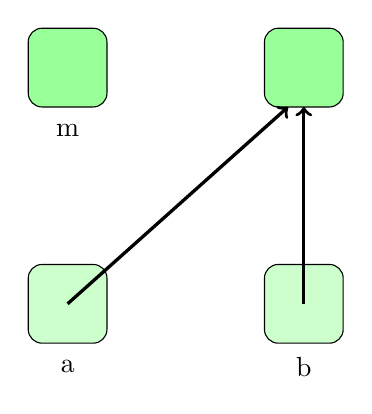
\begin{tikzpicture}[scale=1]
        % \draw[help lines, gray!50, very thin] (0,0) grid (4,4);
        % \filldraw[black] (0,0) circle (2pt);
        
        \draw[fill=green!40, rounded corners=5pt] (3,3) rectangle node {\textbf{ }} (4,4);

        \draw[fill=green!40, rounded corners=5pt] (0,3) rectangle node {\textbf{ }} (1,4);
        \node at (0.5,2.7) {m};

        \draw[fill=green!20, rounded corners=5pt] (3,0) rectangle node {\textbf{ }} (4,1);
        \node at (3.5,-0.3) {b};
        \draw[->, very thick] (3.5,0.5) -- (3.5,3);

        \draw[fill=green!20, rounded corners=5pt] (0,0) rectangle node {\textbf{ }} (1,1);
        \node at (0.5,-0.3) {a};
        \draw[->, very thick] (0.5,0.5) -- (3.3,3);
      \end{tikzpicture}      
    \end{column}
  \end{columns}

  \framebreak  

  \begin{columns}
    \begin{column}{.5\textwidth}
      {\texttt
        int m;\\
        int* a;\\
        int* b = malloc(sizeof(int));\\
        a = \&m;\\
        a = b;\\
        m = 10;\\
      }
    \end{column}
    \begin{column}{.5\textwidth}
      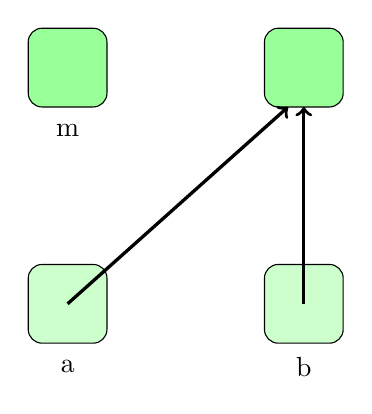
\begin{tikzpicture}[scale=1]
        % \draw[help lines, gray!50, very thin] (0,0) grid (4,4);
        % \filldraw[black] (0,0) circle (2pt);
        
        \draw[fill=green!40, rounded corners=5pt] (3,3) rectangle node {\textbf{ }} (4,4);

        \draw[fill=green!40, rounded corners=5pt] (0,3) rectangle node {\textbf{ }} (1,4);
        \node at (0.5,2.7) {m};

        \draw[fill=green!20, rounded corners=5pt] (3,0) rectangle node {\textbf{ }} (4,1);
        \node at (3.5,-0.3) {b};
        \draw[->, very thick] (3.5,0.5) -- (3.5,3);

        \draw[fill=green!20, rounded corners=5pt] (0,0) rectangle node {\textbf{ }} (1,1);
        \node at (0.5,-0.3) {a};
        \draw[->, very thick] (0.5,0.5) -- (3.3,3);
      \end{tikzpicture}      
    \end{column}
  \end{columns}

  \framebreak  
  

  \begin{columns}
    \begin{column}{.5\textwidth}
      {\texttt
        int m;\\
        int* a;\\
        int* b = malloc(sizeof(int));\\
        a = \&m;\\
        a = b;\\
        m = 10;\\
      }
    \end{column}
    \begin{column}{.5\textwidth}
      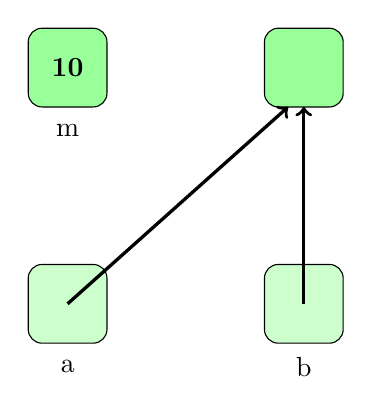
\begin{tikzpicture}[scale=1]
        % \draw[help lines, gray!50, very thin] (0,0) grid (4,4);
        % \filldraw[black] (0,0) circle (2pt);
        
        \draw[fill=green!40, rounded corners=5pt] (3,3) rectangle node {\textbf{ }} (4,4);

        \draw[fill=green!40, rounded corners=5pt] (0,3) rectangle node {\textbf{10}} (1,4);
        \node at (0.5,2.7) {m};

        \draw[fill=green!20, rounded corners=5pt] (3,0) rectangle node {\textbf{ }} (4,1);
        \node at (3.5,-0.3) {b};
        \draw[->, very thick] (3.5,0.5) -- (3.5,3);

        \draw[fill=green!20, rounded corners=5pt] (0,0) rectangle node {\textbf{ }} (1,1);
        \node at (0.5,-0.3) {a};
        \draw[->, very thick] (0.5,0.5) -- (3.3,3);
      \end{tikzpicture}      
    \end{column}
  \end{columns}

  \framebreak  

  \begin{columns}
    \begin{column}{.5\textwidth}
      {\texttt
        int m;\\
        int* a;\\
        int* b = malloc(sizeof(int));\\
        a = \&m;\\
        a = b;\\
        m = 10;\\
        *b = m + 2;
      }
    \end{column}
    \begin{column}{.5\textwidth}
      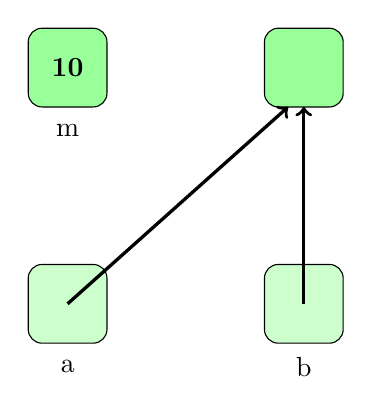
\begin{tikzpicture}[scale=1]
        % \draw[help lines, gray!50, very thin] (0,0) grid (4,4);
        % \filldraw[black] (0,0) circle (2pt);
        
        \draw[fill=green!40, rounded corners=5pt] (3,3) rectangle node {\textbf{ }} (4,4);

        \draw[fill=green!40, rounded corners=5pt] (0,3) rectangle node {\textbf{10}} (1,4);
        \node at (0.5,2.7) {m};

        \draw[fill=green!20, rounded corners=5pt] (3,0) rectangle node {\textbf{ }} (4,1);
        \node at (3.5,-0.3) {b};
        \draw[->, very thick] (3.5,0.5) -- (3.5,3);

        \draw[fill=green!20, rounded corners=5pt] (0,0) rectangle node {\textbf{ }} (1,1);
        \node at (0.5,-0.3) {a};
        \draw[->, very thick] (0.5,0.5) -- (3.3,3);
      \end{tikzpicture}      
    \end{column}
  \end{columns}

  \framebreak  

  \begin{columns}
    \begin{column}{.5\textwidth}
      {\texttt
        int m;\\
        int* a;\\
        int* b = malloc(sizeof(int));\\
        a = \&m;\\
        a = b;\\
        m = 10;\\
        *b = m + 2;
      }
    \end{column}
    \begin{column}{.5\textwidth}
      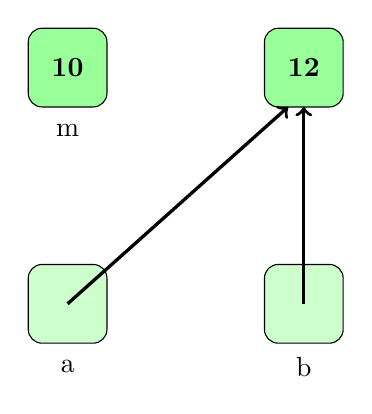
\begin{tikzpicture}[scale=1]
        % \draw[help lines, gray!50, very thin] (0,0) grid (4,4);
        % \filldraw[black] (0,0) circle (2pt);
        
        \draw[fill=green!40, rounded corners=5pt] (3,3) rectangle node {\textbf{12}} (4,4);

        \draw[fill=green!40, rounded corners=5pt] (0,3) rectangle node {\textbf{10}} (1,4);
        \node at (0.5,2.7) {m};

        \draw[fill=green!20, rounded corners=5pt] (3,0) rectangle node {\textbf{ }} (4,1);
        \node at (3.5,-0.3) {b};
        \draw[->, very thick] (3.5,0.5) -- (3.5,3);

        \draw[fill=green!20, rounded corners=5pt] (0,0) rectangle node {\textbf{ }} (1,1);
        \node at (0.5,-0.3) {a};
        \draw[->, very thick] (0.5,0.5) -- (3.3,3);
      \end{tikzpicture}      
    \end{column}
  \end{columns}

  \framebreak
  
  \begin{columns}
    \begin{column}{.5\textwidth}
      {\texttt
        int m;\\
        int* a;\\
        int* b = malloc(sizeof(int));\\
        a = \&m;\\
        a = b;\\
        m = 10;\\
        *b = m + 2;\\
        free(b);
      }
    \end{column}
    \begin{column}{.5\textwidth}
      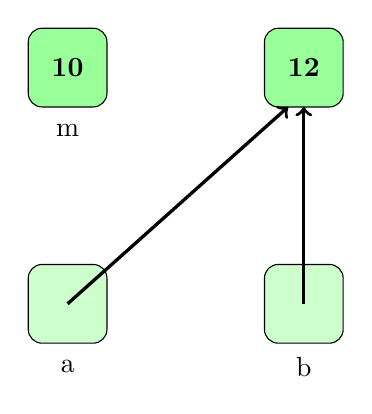
\begin{tikzpicture}[scale=1]
        % \draw[help lines, gray!50, very thin] (0,0) grid (4,4);
        % \filldraw[black] (0,0) circle (2pt);
        
        \draw[fill=green!40, rounded corners=5pt] (3,3) rectangle node {\textbf{12}} (4,4);

        \draw[fill=green!40, rounded corners=5pt] (0,3) rectangle node {\textbf{10}} (1,4);
        \node at (0.5,2.7) {m};

        \draw[fill=green!20, rounded corners=5pt] (3,0) rectangle node {\textbf{ }} (4,1);
        \node at (3.5,-0.3) {b};
        \draw[->, very thick] (3.5,0.5) -- (3.5,3);

        \draw[fill=green!20, rounded corners=5pt] (0,0) rectangle node {\textbf{ }} (1,1);
        \node at (0.5,-0.3) {a};
        \draw[->, very thick] (0.5,0.5) -- (3.3,3);
      \end{tikzpicture}      
    \end{column}
  \end{columns}

  \framebreak

  \begin{columns}
    \begin{column}{.5\textwidth}
      {\texttt
        int m;\\
        int* a;\\
        int* b = malloc(sizeof(int));\\
        a = \&m;\\
        a = b;\\
        m = 10;\\
        *b = m + 2;\\
        free(b);
      }
    \end{column}
    \begin{column}{.5\textwidth}
      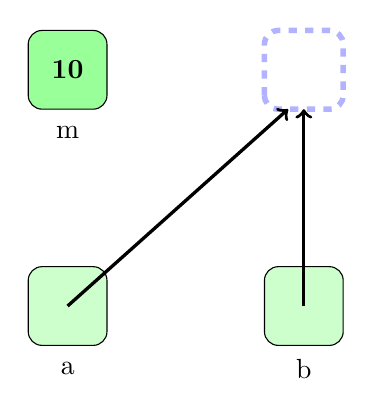
\begin{tikzpicture}[scale=1]
        % \draw[help lines, gray!50, very thin] (0,0) grid (4,4);
        % \filldraw[black] (0,0) circle (2pt);
        
        \draw[blue!30, dashed, line width=2pt, rounded corners=5pt] (3,3) rectangle node {\textbf{ }} (4,4);

        \draw[fill=green!40, rounded corners=5pt] (0,3) rectangle node {\textbf{10}} (1,4);
        \node at (0.5,2.7) {m};

        \draw[fill=green!20, rounded corners=5pt] (3,0) rectangle node {\textbf{ }} (4,1);
        \node at (3.5,-0.3) {b};
        \draw[->, very thick] (3.5,0.5) -- (3.5,3);

        \draw[fill=green!20, rounded corners=5pt] (0,0) rectangle node {\textbf{ }} (1,1);
        \node at (0.5,-0.3) {a};
        \draw[->, very thick] (0.5,0.5) -- (3.3,3);
      \end{tikzpicture}      
    \end{column}
  \end{columns}

  \framebreak

  \begin{columns}
    \begin{column}{.5\textwidth}
      {\texttt
        int m;\\
        int* a;\\
        int* b = malloc(sizeof(int));\\
        a = \&m;\\
        a = b;\\
        m = 10;\\
        *b = m + 2;\\
        free(b);\\
        *a = 11;
      }
    \end{column}
    \begin{column}{.5\textwidth}
      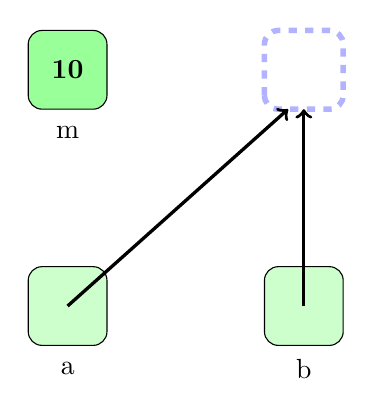
\begin{tikzpicture}[scale=1]
        % \draw[help lines, gray!50, very thin] (0,0) grid (4,4);
        % \filldraw[black] (0,0) circle (2pt);
        
        \draw[blue!30, dashed, line width=2pt, rounded corners=5pt] (3,3) rectangle node {\textbf{ }} (4,4);

        \draw[fill=green!40, rounded corners=5pt] (0,3) rectangle node {\textbf{10}} (1,4);
        \node at (0.5,2.7) {m};

        \draw[fill=green!20, rounded corners=5pt] (3,0) rectangle node {\textbf{ }} (4,1);
        \node at (3.5,-0.3) {b};
        \draw[->, very thick] (3.5,0.5) -- (3.5,3);

        \draw[fill=green!20, rounded corners=5pt] (0,0) rectangle node {\textbf{ }} (1,1);
        \node at (0.5,-0.3) {a};
        \draw[->, very thick] (0.5,0.5) -- (3.3,3);
      \end{tikzpicture}      
    \end{column}
  \end{columns}

  \framebreak

  \begin{columns}
    \begin{column}{.5\textwidth}
      {\texttt
        int m;\\
        int* a;\\
        int* b = malloc(sizeof(int));\\
        a = \&m;\\
        a = b;\\
        m = 10;\\
        *b = m + 2;\\
        free(b);\\
        *a = 11;
      }
    \end{column}
    \begin{column}{.5\textwidth}
      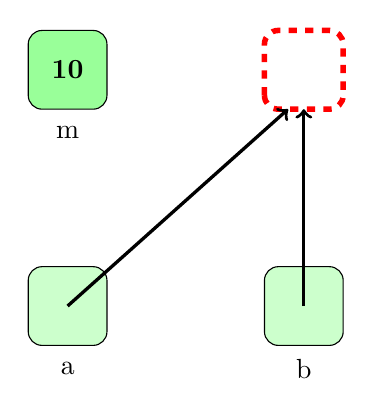
\begin{tikzpicture}[scale=1]
        % \draw[help lines, gray!50, very thin] (0,0) grid (4,4);
        % \filldraw[black] (0,0) circle (2pt);
        
        \draw[red, dashed, line width=2pt, rounded corners=5pt] (3,3) rectangle node {\textbf{ }} (4,4);

        \draw[fill=green!40, rounded corners=5pt] (0,3) rectangle node {\textbf{10}} (1,4);
        \node at (0.5,2.7) {m};

        \draw[fill=green!20, rounded corners=5pt] (3,0) rectangle node {\textbf{ }} (4,1);
        \node at (3.5,-0.3) {b};
        \draw[->, very thick] (3.5,0.5) -- (3.5,3);

        \draw[fill=green!20, rounded corners=5pt] (0,0) rectangle node {\textbf{ }} (1,1);
        \node at (0.5,-0.3) {a};
        \draw[->, very thick] (0.5,0.5) -- (3.3,3);
      \end{tikzpicture}      
    \end{column}
  \end{columns}
  
\end{frame}

\begin{frame}[allowframebreaks,fragile]{copia de string}

  Voltando ao problema de copiar uma string.

  Precisamos na verdade, criar uma nova região na memória para
  armazenar os bytes necessários para a cópia.

  \framebreak

  \lstinputlisting[style=normalc,caption=src/copy0.c]{src/copy0.c}

  \framebreak

  \lstinputlisting[style=normalc,caption=src/copy1.c]{src/copy1.c}

  \framebreak

  \lstinputlisting[style=normalc,caption=src/copy2.c]{src/copy2.c}

  \framebreak

  \begin{center}
    
\includegraphics[width=.8\textwidth]{s_t_malloc.png}
  \end{center}

  Alocamos um espaço de memória \ilcode{0x456} e fizemos \ilcode{t}
  apontar para ele. Copiamos os bytes entre as regiões com o
  \textbf{strcpy}.

\end{frame}


\end{document}

%%% Local Variables:
%%% mode: latex
%%% TeX-master: t
%%% End:
